\RequirePackage{docswitch}
% \flag is set by the user, through the makefile:
%    make note
%    make apj
% etc.
\setjournal{\flag}

\documentclass[\docopts]{\docclass}

% You could also define the document class directly
%\documentclass[]{emulateapj}

% Custom commands from LSST DESC, see texmf/styles/lsstdesc_macros.sty
\usepackage{lsstdesc_macros}

\usepackage{graphicx}
\graphicspath{{./}{./figures/}}
\bibliographystyle{apj}

% Add your own macros here:



% ======================================================================

\begin{document}

\title{TJPCosmo: The DESC Joint Probes Likelihood Pipeline}

\maketitlepre

\begin{abstract}

  This note describes, TJPCosmo, the joint probes likelihood pipeline for LSST DESC. The pipeline is to be used by all DESC Working Groups to produce cosmological constraints from LSST summary data. {\it Host Working Group:} TJP.

\end{abstract}

% Keywords are ignored in the LSST DESC Note style:
\dockeys{}

\maketitlepost

% ----------------------------------------------------------------------
% 

\section{Introduction}
\label{sec:intro}

Overview, need for a joint-likelihood pipeline in the context of LSST.

% ----------------------------------------------------------------------

\section{Pipeline structure}
\label{sec:struct}

From pipelines repo. Include pipeline diagram - Figure \ref{fig:diagram}.

\begin{figure}
  \centering
  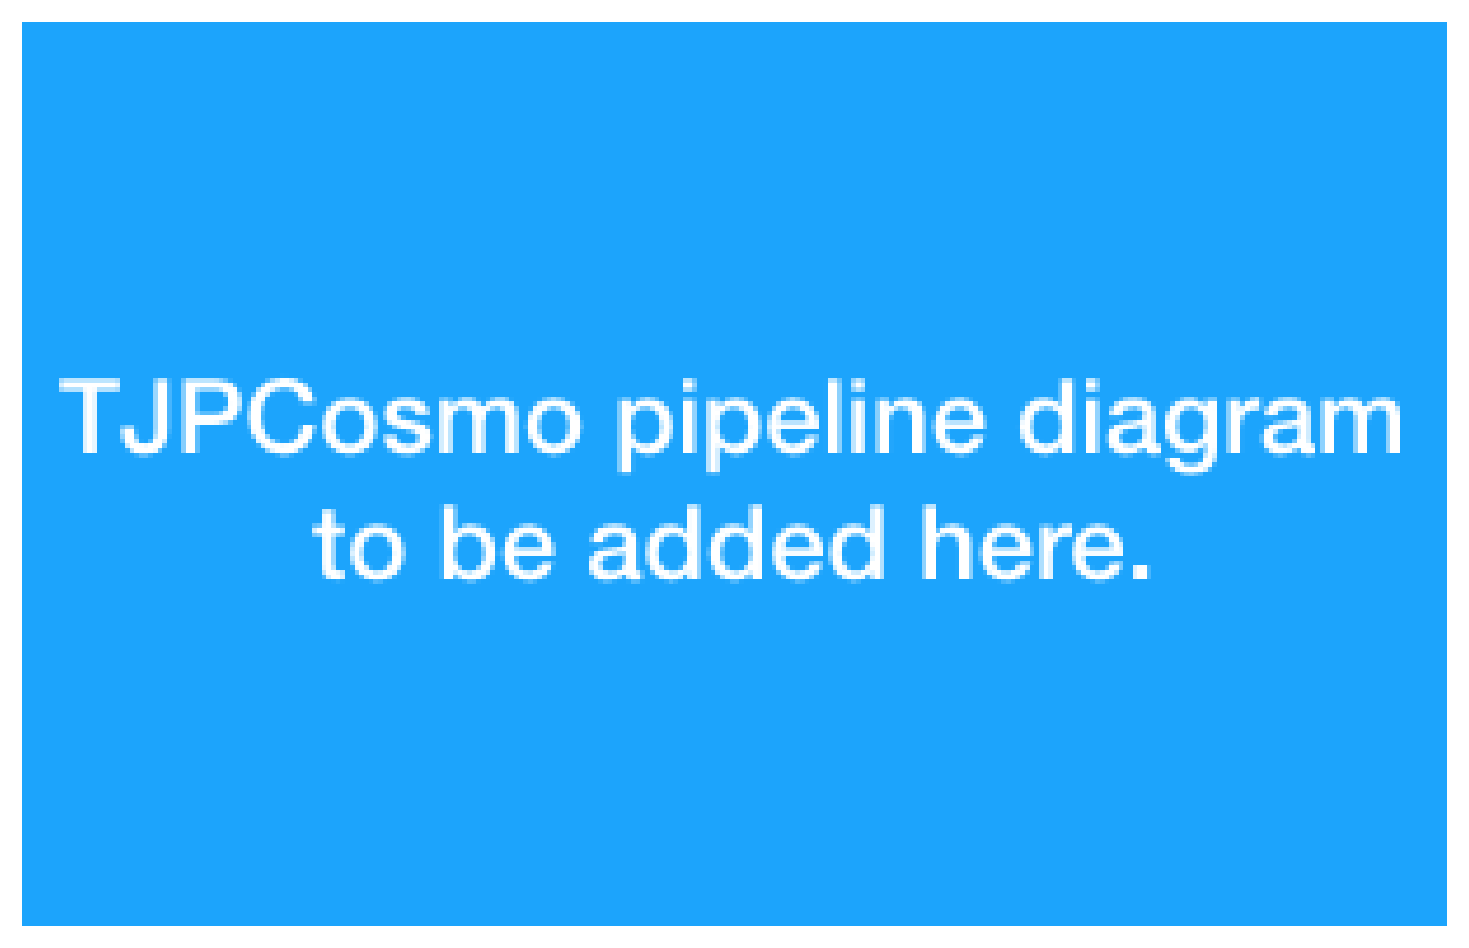
\includegraphics[width=0.49\textwidth]{tjpcosmo_diagram.eps}
  \caption{TJPCosmo pipeline diagram goes here.}
  \label{fig:diagram}
\end{figure}

% ----------------------------------------------------------------------

\section{Analysis stages}
\label{sec:analysis}


\begin{table}[h!]
    \caption{Example analysis stage.}
    \label{tab:stage1}
    \begin{tabular}{| l| l |}
      \hline
      Name & x\\\hline
      Description & x\\\hline
      Inputs & x\\\hline
      Outputs & x\\\hline
      Parallel size & x\\\hline
      Run time & x\\\hline
      I/O dominant? & x\\\hline
      Dependencies & x\\\hline
      Future & x\\\hline
      Notes & x\\\hline
    \end{tabular}
\end{table}
% ----------------------------------------------------------------------

\section{Data}
\label{sec:data}

\begin{table}[h!]
    \caption{Example data.}
    \label{tab:stage1}
    \begin{tabular}{| l| l |}
      \hline
      Name & x\\\hline
      Description & x\\\hline
      Format & x\\\hline
      Data & x\\\hline
      Metadata & x\\\hline
      Size & x\\\hline
      Notes & x\\\hline
    \end{tabular}
\end{table}

% ----------------------------------------------------------------------

\section{External infraestructure}
\label{sec:ext}
% ----------------------------------------------------------------------

\section{Unit tests, System tests and Validation tests}
\label{sec:tests}


% ----------------------------------------------------------------------

\section{Milestones}
\label{sec:mile}

\begin{table}[h!]
    \caption{TJPCosmo milestones.}
    \label{tab:mile}
    \begin{tabular}{| l| l |}
      \hline
      \textbf{Date} & \textbf{Milestone}\\
      \hline
      xx/xx & Task\\
      xx/xx & Task\\
      xx/xx & Task\\
      \hline
    \end{tabular}
\end{table}


% ----------------------------------------------------------------------

\section{Future plans}
\label{sec:future}

Future features.
% ----------------------------------------------------------------------

\subsection*{Acknowledgments}

%%% Here is where you should add your specific acknowledgments, remembering that some standard thanks will be added via the \code{desc-tex/ack/*.tex} and \code{contributions.tex} files.

%This paper has undergone internal review in the LSST Dark Energy Science Collaboration. % REQUIRED if true

%\input{contributions} % Standard papers only: author contribution statements. For examples, see http://blogs.nature.com/nautilus/2007/11/post_12.html

% This work used TBD kindly provided by Not-A-DESC Member and benefitted from comments by Another Non-DESC person.

% Standard papers only: A.B.C. acknowledges support from grant 1234 from ...

%\input{desc-tex/ack/standard} % also available: key standard_short

% This work used some telescope which is operated/funded by some agency or consortium or foundation ...

% We acknowledge the use of An-External-Tool-like-NED-or-ADS.

%{\it Facilities:} \facility{LSST}

% Include both collaboration papers and external citations:
\bibliography{main,lsstdesc}

\end{document}

% ======================================================================
